\documentclass[12pt,a4paper]{article}

% Basic Packages
\usepackage[utf8]{inputenc}
\usepackage[T1]{fontenc}
\usepackage{geometry}
\usepackage{graphicx}
\usepackage{microtype}
\usepackage{subfiles}
\usepackage{enumitem}
\usepackage{lipsum}
\usepackage{tikz-cd}
\usepackage{pifont}  % For Pifont symbols

% Mathematics Packages
\usepackage{amsmath, amssymb, amsthm}
\usepackage{mathtools}
\numberwithin{equation}{section}

% For improved tables
\usepackage{booktabs}

% For improved referencing
\usepackage{hyperref}

% Custom theorem environments
\newtheorem{theorem}{Theorem}[section]
\newtheorem{lemma}[theorem]{Lemma}
\newtheorem{corollary}[theorem]{Corollary}
\newtheorem{proposition}[theorem]{Proposition}
\newtheorem{definition}[theorem]{Definition}
\newtheorem{remark}[theorem]{Remark}
\newtheorem{example}[theorem]{Example}

\renewcommand\epsilon{\ensuremath{\varepsilon}}

% Page geometry (adjust margins as needed)
\geometry{
  left=25mm,
  right=25mm,
  top=25mm,
  bottom=25mm
}

% Title, author, and date
\title{Reflective Subcategories}
% \author{Author Name}
\date{\today} % or specify a date manually

\begin{document}

\maketitle % Print the title
\tableofcontents

\section{Introduction} % (fold)
\label{sec:Introduction}
In this mini project we study reflective subcategories and their properties. To motivate this a little bit, consider the category of abelian groups which are contained in the category of groups. The abelianization functor then serves as a left adjoint to this inclusion. We can then consider the monad induced by this adjunction and ask ourselves if the category of $ T $-algebras on groups ($ T $ being the monad) is equivalent to the category of abelian groups. As we shall see, this is indeed the case, and it follows from the result that the inclusion of a reflective subcategory is monadic.

We\footnote{``We'' is used only as a literary device, as this is solely my own work.} have chosen to answer the questions that accompany this mini project as an extended text which we have tried to fit together in a logical manner. Section~\ref{sec:Preliminaries} answers questions 1--4 while section~\ref{sec:Monadic Structure of Reflective Subcategories} answers question 5. More specifically, we have the map between questions and theorems/propositions/lemmas as shown in Figure~\ref{fig:map}.
\begin{figure}[ht]
  \begin{center}
    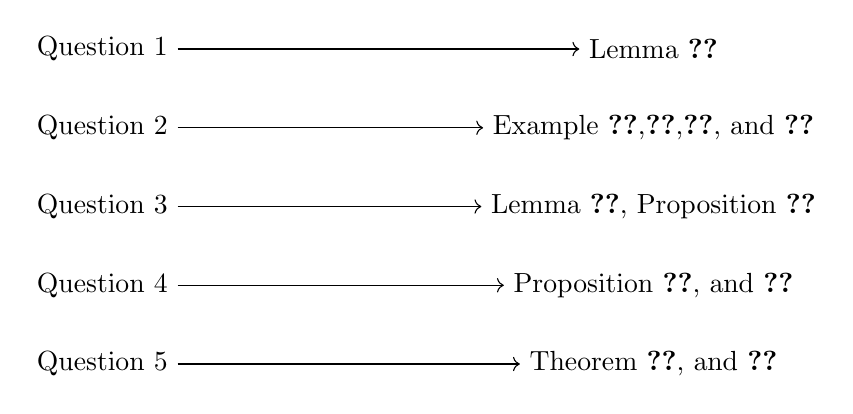
\begin{tikzpicture}
      \node (Q1) at (0,4) {Question 1};
      \node (Q2) at (0,3) {Question 2};
      \node (Q3) at (0,2) {Question 3};
      \node (Q4) at (0,1) {Question 4};
      \node (Q5) at (0,0) {Question 5};
      \node (A1) at (7,4) {Lemma~\ref{lem:adjprops}};
      \node (A2) at (7,3) {Example~\ref{ex:ab},\ref{ex:ring},\ref{ex:met}, and \ref{ex:haus}};
      \node (A3) at (7,2) {Lemma~\ref{lem:ess}, Proposition~\ref{prop:local}};
      \node (A4) at (7,1) {Proposition~\ref{prop:creates}, and~\ref{prop:colims}};
      \node (A5) at (7,0) {Theorem~\ref{thm:beck}, and~\ref{thm:converse}};
      \draw[->] (Q1) -- (A1);
      \draw[->] (Q2) -- (A2);
      \draw[->] (Q3) -- (A3);
      \draw[->] (Q4) -- (A4);
      \draw[->] (Q5) -- (A5);
      % Add more nodes and arrows as needed
    \end{tikzpicture}
  \end{center}
  \caption{Correspondence between questions in the mini project problem sheet and the appropriate results in this text.}\label{fig:map}
\end{figure}

% section Introduction (end)

\section{Preliminaries} % (fold)
\label{sec:Preliminaries}
We start by reviewing some basic results about adjoint functors, as well as their definition.
\begin{definition}
  Given two functors $ F:\mathcal{C} \rightleftarrows \mathcal{D}:G $ we say that $ F $ is left adjoint to $ G $, written as $ F \dashv G $, if there exists a pair of natural transformations
  \begin{align*}
    &\eta: 1_\mathcal{C} \implies GF \\
    &\epsilon: FG \implies 1_{\mathcal{D}}
  \end{align*}
  which makes the following diagrams commute
\[\begin{tikzcd}
	& FGF &&& GFG \\
	F && F & G && G.
	\arrow["{1_F}"', from=2-1, to=2-3, Rightarrow]
	\arrow["{\eta F}", from=2-1, to=1-2, Rightarrow]
	\arrow["F\varepsilon", from=1-2, to=2-3, Rightarrow]
	\arrow["{1_G}"', from=2-4, to=2-6, Rightarrow]
	\arrow["G\eta", from=2-4, to=1-5, Rightarrow]
	\arrow["{\varepsilon G}", from=1-5, to=2-6, Rightarrow]
\end{tikzcd}\]
\end{definition}

\begin{lemma}
  \label{lem:adjprops}
  If  $ F \dashv G $ is a pair of adjoint functors with unit $ \eta: 1_\mathcal{C} \implies GF $ and counit $ \epsilon: FG \implies 1_\mathcal{D} $ then
  \begin{enumerate}[label=(\roman*)]
    \item $ G $ is faithful if and only if each component of $ \epsilon $ is an epimorphism.
    \item $ G $ if full if and only if each component of $ \epsilon $ is a split monomorphism.
    \item $ G $ is fully faithful if and only if $ \epsilon $ is an isomorphism.
    \item $ F $ is faithful if and only if each component of $ \eta $ is a monomorphism.
    \item $ F $ is full if and only if each component of $ \eta $ is a split epimorphism.
    \item $ F $ is fully faithful if and only if $ \eta $ is an isomorphism.
  \end{enumerate}
\end{lemma}
\begin{proof}
  Notice that statements (\textit{iv})--(\textit{vi}) are dual of statements (\textit{i})--(\textit{iii}) and hence it suffices to only show the first three statements and then argue by duality. We will do this argumentation quite explicit and show how the dual argument follows from the original argument.
  \begin{enumerate}[label=(\roman*)]
    \item ($ \implies $): Assume that $ G $ is faithful. Let $ d,d' \in \mathcal{D} $ and $ g_1, g_2 \in \text{Hom}_{\mathcal{D}}(FGd, d') $ be so that
      \begin{equation}
        g_1 \circ \epsilon_d = g_2 \circ \epsilon_d
      .\end{equation}
      We want to show that $ g_1 = g_2 $. From the commutativity of the following triangle
      \[\begin{tikzcd}
	& GFGd \\
	      Gd && Gd
	      \arrow["{G\varepsilon_{d}}", from=1-2, to=2-3]
	      \arrow["{\eta_{Gd}}", from=2-1, to=1-2]
	      \arrow["{1_{Gd}}"', from=2-1, to=2-3]
      \end{tikzcd}\]
      we have that $ G\epsilon_d $ is an epimorphism. From this we have the following series of equivalent statements
      \begin{align*}
        g_1 \circ \epsilon_d &= g_2 \circ \epsilon_d \quad \text{iff} \\
        G(g_1 \circ \epsilon_d) &= G(g_2 \circ \epsilon_d) \quad \text{iff} \\
        Gg_1 \circ G\epsilon_d &= Gg_2 \circ G\epsilon_d\quad \text{iff} \\
        Gg_1 &= Gg_2 \quad \text{iff} \\
        g_1 &= g_2
      \end{align*}
      where the first and last equivalence follows since $ G $ is faithful.

      \noindent ($ \impliedby $): Suppose $ \epsilon $ is an epimorphism, i.e., each component $ \epsilon_d $ is an epimorphism. Let $ g_1, g_2 \in \text{Hom}_{\mathcal{D}}(d, d') $ such that $ Gg_1 = Gg_2 $. We want to show that $ g_1 = g_2 $. Let $ FGg: FGd \to FGd' $ denote the same morphism $ FGg_1 = FGg_2 $. Since $ \epsilon $ is a natural transformation, we have the commutative diagram
      \[\begin{tikzcd}
	      FGd & {FGd'} \\
	      d & {d'}
	      \arrow["{\varepsilon_d}"', from=1-1, to=2-1]
	      \arrow["FGf", from=1-1, to=1-2]
	      \arrow["{\varepsilon_{d'}}", from=1-2, to=2-2]
	      \arrow["{g_2}", from=2-1, to=2-2, shift left=2, "\phantom{aa}"'{name=U, below}] % Shifted left with label above
	      \arrow["{g_1}"', from=2-1, to=2-2, shift right=2, "\phantom{aa}"{name=D, above}] % Shifted right with label below
      \end{tikzcd}\]
      which gives us
      \begin{equation}
        g_1 \circ \epsilon_d = \epsilon_{d'} \circ FGg
      \end{equation}
      and
      \begin{equation}
        g_2 \circ \epsilon_d = \epsilon_{d'} \circ FGg
      \end{equation}
      hence
      \begin{equation}
        g_1 \circ \epsilon_d = g_2 \circ \epsilon_d.
      \end{equation}
      Since $ \epsilon $ is an epimorphism it finally follows that
      \begin{equation}
        g_1 = g_2
      \end{equation}
      as desired.

    \item ($ \implies $): Suppose $ G $ is full. Note that it suffices to find $ \alpha: 1_\mathcal{D} \implies FG $ such that $ \alpha\circ \epsilon = 1_{FG} $. Since $ G $ is full there must exist $ \alpha: 1_\mathcal{D} \implies FG $ such that $ G\alpha = \eta G $. As $ \epsilon $ is a natural transformation we have that
      \begin{align*}
        \alpha \circ \epsilon &= \epsilon FG \circ FG \alpha \\
                              &= \epsilon FG \circ F \eta G
      .\end{align*}
      From the triangle identity for the unit we have that
      \begin{equation}
        \epsilon F \circ F \eta = 1_F
        \label{eq:triunit}
      \end{equation}
      which implies that
      \begin{equation}
        \epsilon FG \circ F \eta G = 1_{FG}
      \end{equation}
      and hence
      \begin{equation}
        \alpha \circ \epsilon = 1_{FG}
      \end{equation}
      showing that $ \epsilon $ is a split monomorphism.


      \noindent ($ \impliedby $): Assume $ \epsilon $ is a split monomorphism and let $ \alpha: 1_{\mathcal{D}} \implies FG $ be the splitting. We then have that
      \begin{equation}
        G\alpha \circ G \epsilon = 1_{GFG}
      \end{equation}
      which, from the triangle identity for $ \epsilon $, implies that
      \begin{equation}
        G\alpha = \eta G.
        \label{eq:alpeta}
      \end{equation}
      Let $ d,d' \in \mathcal{D} $ and $ f \in \text{Hom}_{\mathcal{C}}(Gd, Gd') $. Define
      \begin{equation}
        g = \epsilon_{d'} \circ Ff \circ \alpha_d.
      \end{equation}
      From Equation~\ref{eq:alpeta} and the naturality of $ \eta $ we then have that
      \begin{align*}
        Gg &= G\epsilon_{d'} \circ GFg \circ G\alpha_d \\
           &= G\epsilon_{d'} \circ GFg \circ \eta_{Gd} \\
           &= G\epsilon_{d'} \circ \eta_{Gd'} \circ f \\
           &= f
      \end{align*}
      which shows that $ G $ is full, as desired.


    \item If $ \epsilon $ is an isomorphism then it is a split monomorphism and an epimorphism, so the ($ \impliedby $) direction follows trivially from (\textit{i}) and (\textit{ii}). The ($ \implies $) direction follows by (\textit{i}) and (\textit{ii}) if we can show that a split mono- and epimorphism is an isomorphism. Assume therefore that $ f: x \to y $ is a split mono- and epimorphism in some ambient category $ \mathcal{B} $. Let $ g: y \to x $ be the splitting of $ f $. By assumption we know that $ g\circ f = 1_x $. Moreover
    \begin{equation}
      1_y \circ f = f \circ g \circ f
    \end{equation}
    and since $ f $ is also an epimorphism we have that $ g\circ f = 1_y $. Hence $ f $ is indeed an isomorphism.


  \item This and the next two statements follows by duality. More explicitly, if $ F \dashv G $ then $ G^{\text{op}} \dashv F^{\text{op}} $ with unit $ \epsilon^{\text{op}}: 1_{\mathcal{D}^{\text{op}}} \implies F^{\text{op}}G^{\text{op}} $ and counit $ \eta^{\text{op}}: G^{\text{op}}F^{\text{op}} \implies 1_{\mathcal{C}^{\text{op}}} $. From ($ i $) we therefore have that
    \begin{align*}
      F & \text{ faithful} \\
        &\Updownarrow \\
      F^{\text{op}}& \text{ faithful} \\
                   &\Updownarrow \\
      \eta^{\text{op}} &\text{ is an epimorphism} \\
                       &\Updownarrow \\
      \eta &\text{ is a monomorphism}
    .\end{align*}

  \item We have the following sequence of equivalent statements
    \begin{align*}
      F &\text{ full} \\
        &\Updownarrow \\
      F^{\text{op}} &\text{ full} \\
        &\Updownarrow \\
      \eta^{\text{op}} &\text{ is a split monomorphism} \\
                       &\Updownarrow \\
      \eta &\text{ is a split epimorphism}
    .\end{align*}

  \item We have the following sequence of equivalent statements
    \begin{align*}
      F &\text{ is fully faithful} \\
        &\Updownarrow \\
      F^{\text{op}}  &\text{ is fully faithful} \\
                     &\Updownarrow \\
      \eta^{\text{op}}&\text{ is an isomorphism} \\
                      &\Updownarrow \\
      \eta &\text{ is an isomorphism}
    .\end{align*}
  \end{enumerate}
\end{proof}

\subsection{Reflective subcategory} % (fold)
\label{sub:Reflective subcategories}
The previous lemma will come in handy as we begin our studies of reflective subcategories.
\begin{definition}
Consider an inclusion of a full subcategory $ i: \mathcal{D} \subset \mathcal{C} $. If we have an adjunction $ L \dashv i $ for some functor $ L: \mathcal{C} \to \mathcal{D} $ then we say that $ \mathcal{D} $ is a \textbf{reflective subcategory} of $ \mathcal{C} $ and $ L $ is called the \textbf{reflector}.
\end{definition}

Many well known categories can be thought of as reflective subcategories.

\begin{example}
  \label{ex:ab}
  The subcategory of abelian groups $ \mathbf{Ab} $ is a reflective subcategory of the category of groups $ \mathbf{Grp} $ with reflector $ L:\mathbf{Grp} \to \mathbf{Ab} $ the abelianization functor $ G \mapsto G/[G,G] $. To see this, we must show that $ L \dashv i $ and hence must define the unit and counit. Let $ \eta: 1_{\mathbf{Grp}} \implies iL $ be the projection $ \pi_G: G \to G/[G,G] $ and
  $ \epsilon: Li \implies \mathbf{Ab} $ the identity. We must then verify the triangle identities. Let $ G \in \mathbf{Grp} $, then
  \begin{align*}
    \epsilon_{LG} \circ L\eta_G &= 1_{LG} \circ L\pi_G \\
                                &= L\pi_G \\
                                &= 1_{LG}
  \end{align*}
  where the last equality follows since the abelianization of the projection induced from the abelianization must necessarily be the identity. Let $ A \in \mathbf{Ab} $, then
  \begin{align*}
    i\epsilon_A \circ \eta_{iA} &= 1_{iA} \circ \pi_{iA} \\
                                &= 1_{iA}
  \end{align*}
  as the abelianization of an abelian group is just the same group and hence the projection is the identity.
\end{example}

\begin{example}
  \label{ex:ring}
  The subcategory of commutative rings $ \mathbf{CRing} $ is a reflective subcategory of the category of rings $ \mathbf{Ring} $. We let $ L:\mathbf{Ring} \to \mathbf{CRing} $ be given by $ L(R) = R/[R,R] $ where $ [R,R] $ is the ideal generated by elements of the form $ ab - ba $ for $ a,b \in R $. We let the unit $ \eta: 1_{\mathbf{Ring}} \implies iL $ be the projection $ \eta_R = \pi_R: R \to R/[R,R] $ and the counit is again just the identity $ \epsilon = 1_{\mathbf{CRing}} $. We must then verify the triangle identities. To this end, let $ R \in \mathbf{Ring} $, then
  \begin{align*}
    \epsilon_{LR} \circ L\eta_R &= 1_{LR} \circ L\pi_R \\
                                &= L\pi_R \\
                                &= 1_{LR}
  \end{align*}
  where the last equality again follows by the same reasoning as for groups. The other triangle identity is also shown identically as with group, i.e, for $ R \in \mathbf{CRing} $, we have
  \begin{align*}
    i\epsilon_R \circ \eta_{iR} &= \pi_{iR} \circ 1_{iR} \\
                                &= \pi_{iR} \\
                                &= 1_{iR}
  \end{align*}
  where the last equality follows because the commutator of a commutative group is the zero ideal.
\end{example}

\begin{example}
  \label{ex:met}
  The category of complete metric spaces $ \mathbf{CMet} $ is a reflective subcategory of $ \mathbf{Met} $ (the category of metric spaces). To see this let the reflector $ L:\mathbf{Met} \to \mathbf{CMet} $ be the completion operation $ M \mapsto \widehat{M} $ of a metric space. Now, there is a canonical uniformly continuous map $ \iota_M: M \to \widehat{M} $ which has the universal property that if $ N $ is any other complete metric space and $ f: M \to N $ is a uniformly continuous map, then there exists a unique uniformly continuous map $ \tilde{f}:\widehat{M} \to N $ such that $ \tilde{f}\circ \iota = f $.

  Note also that a complete metric space $ N $ is uniquely isomorphic to its completion $ \widehat{N} $. Hence, let the unit $ \eta: 1_{\mathbf{Met}} \implies iL $ be $ \iota $ and the counit $ \epsilon: Li \implies 1_{\mathbf{CMet}} $ the inverse of $ \iota $ (which exists on $ \mathbf{CMet} $ by the earlier remark). The details of checking the naturality of $ \eta $ and $ \epsilon $ are straightforward and we leave it to the interested reader. Now,
  \begin{align*}
    \epsilon_{LM} \circ L\eta_M &= \iota^{-1}_{\widehat{M}} \circ L\iota_M \\
                                &= \iota^{-1}_{\widehat{M}} \circ \iota_{\widehat{M}} \\
                                &= 1_{\widehat{M}}
  \end{align*}
  and
  \begin{align*}
    i\epsilon_N \circ \eta_{iN} &= \iota^{-1}_{iN} \circ \iota_{iN} \\
                                &= 1_{iN}
  \end{align*}
  showing that $ \eta $ and $ \iota $ satisfy the requirement for being a unit and counit respectively.
\end{example}

\begin{example}[\cite{riehl2017category}]
  \label{ex:haus}
  The category of compact Hausdorff spaces, denoted by $ \mathbf{cHaus} $, is a reflective category of \textbf{Top}, the category of topological spaces. To see this, let the reflector $ L=\beta $ be the functor which sends a topological space to its Stone-\v Cech compactification. This has the universal property that if $ f: X \to K $ is any map from $ X $ into a compact Hausdorff space $ K $, the $ f $ factors uniquely through $ \beta X $. Let the unit be the canonical embedding $ \eta_X: X \to \beta X $ and the counit the unique isomorphism from a compact Hausdorff space $ K $ to $ \beta K $. Thinking of the isomorphism $ \epsilon $ as the identity the triangle identities just says that
  \begin{align*}
    \beta \eta_X &= 1_{\beta X} \\
    \eta_{K} &= 1_{K}
  \end{align*}
  which both holds as the Stone-\v Cech compactification of the map $ X \to \beta X $ is a unique isomorphism, and the same goes for $ \eta_K $.
\end{example}

Before establishing more general results about reflective subcategories, we need a technical lemma.
\begin{lemma}
  \label{lem:com}
  For a reflective subcategory $ i:\mathcal{D} \subset \mathcal{C} $ with reflector $ L: \mathcal{D} \to \mathcal{C} $ we have that if $ c \in \mathcal{C} $, then $ \eta_{iLc} = iL\eta_c $.
\end{lemma}
\begin{proof}
  Let $ c \in \mathcal{C} $. From the triangle equality we have that
  \begin{equation}
    \epsilon_{Lc} \circ L\eta_c = 1_{Lc}
  \end{equation}
  which implies
  \begin{equation}
    i\epsilon_{Lc} \circ iL\eta_c = 1_{iLc}.
  \end{equation}
  The other triangle equality gives
  \begin{equation}
    i\epsilon_{Lc} \circ \eta_{iLc} = 1_{iLc}.
  \end{equation}
  which combined gives
  \begin{equation}
    i\epsilon_{Lc} \circ \eta_{iLc} = i\epsilon_{Lc} \circ iL\eta_{c}.
  \end{equation}
  From Lemma~\ref{lem:adjprops} (iii) we have that $ \epsilon_{Lc} $ is invertible and hence $ i\epsilon_{Lc} $ is also invertible. This gives
  \begin{align*}
    i\epsilon_{Lc} \circ \eta_{iLc} &= i\epsilon_{Lc} \circ iL\eta_{c} \\
                                    &\Updownarrow \\
    (i\epsilon_{Lc})^{-1} \circ i\epsilon_{Lc} \circ \eta_{iLc} &= (i\epsilon_{Lc})^{-1} \circ i\epsilon_{Lc} \circ iL\eta_{c} \\
                                                                &\Updownarrow \\
    \eta_{iLc} &= iL\eta_c
  \end{align*}
  which was what we wanted to show.
\end{proof}
% subsection Reflective subcategories (end)

\subsection{Properties of reflective subcategories} % (fold)
\label{sub:Properties of reflective subcategories}
The condition of being a reflective subcategory allows us to say something about the unit $ \eta: 1_\mathcal{C} \implies iL $:
\begin{lemma}
  \label{lem:ess}
  For a reflective subcategory $ i:\mathcal{D} \subset \mathcal{C} $ with reflector $ L: \mathcal{D} \to \mathcal{C} $ we have that an object $ c \in \mathcal{C} $ is in the essential image of $ i $ if and only if $ \eta_c: c \to iLc $ is an isomorphism.
\end{lemma}
\begin{proof}
  As the $ \impliedby $ direction is trivially true we only need to show the $ \implies $ direction. Suppose therefore that $ c \in \mathcal{C} $ is in the essential image of $ i $. This means that there exist an isomorphism $ f: c \to id $ for some $ d \in \mathcal{D} $. Define $ \alpha: iLc \to c $ by $ \alpha = f^{-1} \circ i(\epsilon_d \circ Lf) \in \text{Hom}_{\mathcal{C}}(iLc, c) $. Note that since $ i $ is fully faithful we have by Lemma~\ref{lem:adjprops} (\textit{iii}) that $ \epsilon $ is an isomorphism and hence, by one of the triangle identities, $ \eta_{id} $ must be the inverse of $ i\epsilon_d $. Keeping this in mind we have
  \begin{align*}
    \eta_c \circ \alpha &= \eta_c \circ f^{-1} \circ i(\epsilon_d \circ Lf) \\
                        &= iLf^{-1} \circ \eta_{id} \circ i\epsilon_{d} \circ iLf \\
                        &= (iLf)^{-1} \circ iLf \\
                        &= 1_{iLc}.
  \end{align*}
  We also have that
  \begin{align*}
    \alpha \circ \eta_c &= f^{-1} \circ i(\epsilon_d \circ Lf) \circ \eta_c \\
                        &= f^{-1} \circ i\epsilon_d \circ \eta_{id} \circ f \\
                        &= f^{-1} \circ f \\
                        &= 1_c
  \end{align*}
  where the second equality follows from the naturality of $ \eta $ and the third equality follows from one of the triangle identities for the adjunction. Thus we see that an object $ c \in \mathcal{C} $ is in the essential image of $ i $ if and only if $ \eta_c $ is an isomorphism as desired.
\end{proof}

We can actually say something more concretely about the essential image of $ i $:
\begin{proposition}
  \label{prop:local}
  Given a reflective subcategory $ i: \mathcal{D} \subset \mathcal{C} $ with reflector $ L: \mathcal{C} \to \mathcal{D} $ the essential image of $ i $ consists of the objects $ c \in \mathcal{C} $ that are local in the following sense: the pre-composition functions $ f^{*}:\text{Hom}_{\mathcal{C}}(b, c) \to \text{Hom}_{\mathcal{C}}(a, c) $ are isomorphisms for all $ f: a \to b \in \text{Hom}_{\mathcal{C}}(a, b) $ for which $ Lf: La \to Lb \in \text{Hom}_{\mathcal{D}}(La, Lb) $ is an isomorphism.
\end{proposition}
\begin{proof}
  Let $ c \in \mathcal{C} $ be in the essential image of $ i $. Let $ a,b \in \mathcal{C} $ and assume $ f: a \to b $ is a morphism such that $ Lf: La \to Lb $ is an isomorphism. We want to show that $ f^{*} $ is an isomorphism.

  \textit{Injectivity}. Let $ g,g': b \to c $ be such that $ g\circ f = g'\circ f $. This implies that $ Lg \circ Lf = Lg' \circ Lf $ and since $ Lf $ is an isomorphism we have that $ Lg = Lg' $. Using the previous lemma we have that $ \eta_{iLc} $ is an isomorphism and hence we have
  \begin{align*}
    Lg &= Lg' \\
       &\Downarrow \\
    \eta^{-1}_{iLc}\circ iLg \circ \eta_b &= \eta^{-1}_{iLc} \circ iLg' \circ \eta_b \\
                                     &\Updownarrow \\
    \eta^{-1}_{iLc} \circ \eta_{iLc} \circ g &= \eta^{-1}_{iLc} \circ \eta_{iLc} \circ g' \\
                                             &\Updownarrow \\
    g &= g'
  \end{align*}
  which shows that $ f^{*} $ is injective.

  \textit{Surjectivity}. Let $ h \in \text{Hom}_{\mathcal{C}}(a, c) $. Define
  \begin{equation}
    g = \eta^{-1}_c \circ iLh \circ (iLf)^{-1} \circ \eta_b
  \end{equation}
  which is well defined as both $ \eta_c $ and $ \eta_{iLc} $ are invertible (invertibility of $ iLf $ follows since $ Lf $ is invertible). We then have that
  \begin{align*}
    f^*(g) &= \eta^{-1}_c \circ iLh \circ \underbrace{(iLf)^{-1} \circ \eta_b \circ f}_{\eta_a} \\
           &= \eta^{-1}_c \circ \underbrace{iLh \circ \eta_a}_{\eta_{c} \circ h} \\
           &= \eta^{-1}_c \circ \eta_c \circ h \\
           &= h
  .\end{align*}
  Hence $ f^{*} $ is surjective which together with the previous part means it is and isomorphism.

  Conversely, assume that $ f^*:\text{Hom}_{\mathcal{C}}(b,c) \to \text{Hom}_{\mathcal{C}}(a, c) $ is an isomorphism whenever $ Lf: La \to Lb $ is an isomorphism. We want to show that $ c $ is in the essential image of $ i $, which by the previous lemma means it is sufficient to show that $ \eta_c $ is an isomorphism. Since $ i $ is fully faithful we have that $ \epsilon_{Lc} $ is an isomorphism and its inverse must be $ L\eta_c $. This in particular means that $ L\eta_c $ is an isomorphism which by assumption means that $ \eta_c^{*}: \text{Hom}_{\mathcal{C}}(iLc, c) \to \text{Hom}_\mathcal{C}(c, c) $ is an isomorphism. This means there exists an $ \alpha_c \in \text{Hom}_\mathcal{C}(iLc, c) $ such that $ \alpha_c \circ \eta_c = 1_c $. Thus
  \begin{align*}
    iL(\alpha_c \circ \eta_c) &= 1_{iLc} \\
                              &\Updownarrow \\
    iL\alpha_c \circ iL \eta_c &= 1_{iLc}
  \end{align*}
  and by Lemma~\ref{lem:com} this is equivalent to saying
  \begin{equation}
    iL\alpha_c \circ \eta_{iLc} = 1_{iLc}.
  \end{equation}
  Using naturality of $ \eta $ we then have that
  \begin{align*}
    \eta_c \circ \alpha_c &= iL\alpha_c \circ \eta_{iLc} \\
                          &= 1_{iLc}
  \end{align*}
  which shows that $ \alpha_c $ is an inverse to $ \eta_c $ and so $ \eta_c $ is an isomorphism which means that $ c $ is in the essential image of $ i $ as desired.
\end{proof}
% subsection Properties of reflective subcategories (end)

\subsection{Creation of limits} % (fold)
\label{sub:Creation of limits}
We start by reviewing the notions of reflection and creation of limits.
\begin{definition}[Reflection of limits]
  Let $ F: \mathcal{C} \to \mathcal{D} $ be a functor and $ J:I \to \mathcal{C} $ a diagram. We say that $ F $ \textbf{reflects} limits of $ J $ if whenever we have a cone $ \eta: \Delta x \implies J $ over $ J $ for some $ x \in \mathcal{C} $ such that $ F\eta $ is a limit of $ F\circ J $ in $ \mathcal{D} $, then $ \eta $ was already a limit of $ J $ in $ \mathcal{C} $.
\end{definition}
\begin{definition}[Creation of limits]
  Let $ F: \mathcal{C} \to \mathcal{D} $ be a functor between categories and $ J: I \to \mathcal{C} $ a diagram. Suppose the diagram $ F \circ J: I \to \mathcal{D} $ has a limit. We say that $ F $ \textbf{creates} this limit if $ J $ has a limit and $ F $ both preserves and reflects this limit.
\end{definition}
There are of course equivalent notions for the reflection and creation of colimits. Now, the fact that the inclusion functor $ i: \mathcal{D} \subset \mathcal{C} $ of a reflective subcategory is fully faithful has implications in terms of creation of limits:
\begin{proposition}
  \label{prop:creates}
  Let $ i: \mathcal{D} \subset \mathcal{C} $ be a reflective subcategory with reflector $ L:\mathcal{C} \to \mathcal{D} $. The inclusion $ i $ creates all limits that $ \mathcal{C} $ admits.
\end{proposition}
\begin{proof}
  Let $ J: I \to \mathcal{D} $ be a diagram and
  $$ \sigma: \Delta x \implies iJ $$
  a limit cone for some $ x \in \mathcal{C} $. We want to find a limit cone $$ \tau: \Delta z \implies J $$
  such that $ i\tau \cong \sigma $. To do this we first show that
  $$ L\sigma: L\Delta x \implies LiJ $$
  is a limit cone (note that $ L\Delta x = \Delta Lx $) and exploit the fact that $ \epsilon $ is an isomorphism to show that $ \epsilon J \circ L\sigma $ must also be a limit cone. Setting $ z = Lx $ and $ \tau = \epsilon J \circ L\sigma $ finishes the proof. To this end, let
  $$ \delta: \Delta y \implies LiJ $$
  be another cone. We want to find a unique
  $$ \xi: \Delta y \implies L\Delta x $$ such that $ \delta = L\sigma\circ \xi. $

  Remember that $ i $ is fully faithful and hence it is a good idea to work in $ \mathcal{C} $ where we can say something more concrete. With this in mind, take
  $$ i\delta: i\Delta y \implies iLiJ $$
  and vertically compose with
  $$ i\epsilon J: iLiJ \implies iJ $$
  (where $ \epsilon $ is the counit of the adjunction $ L \dashv i $) so that we get
  $$ i\epsilon J \circ i\delta: i\Delta y \implies iJ. $$
  Now, as $ \sigma $ is a limit cone over $ iJ $ we must have that there exists a unique
  $$ \zeta: i\Delta y \implies \Delta x $$
  such that
  $$ \sigma \circ \zeta = i\epsilon J \circ i\delta. $$
  Consider the horizontal composition
  $$ \eta * \zeta: i\Delta y \implies iL \Delta x, $$
  where $ \eta $ is the unit of the adjunction. Since $ i $ is fully faithful there must exist a unique $ \xi: \Delta y \implies L\Delta x $ such that $ i\xi = \eta * \zeta $. We then need to show that $ \delta = L\sigma \circ \xi $, or equivalently (since $ i $ is fully faithful) that $ i\delta = iL\sigma \circ i\xi $. Horizontally pre-composing one of the triangle identities with $ J $ we get the commutative triangle
  \[\begin{tikzcd}
	  & iLiJ \\
	  iJ && iJ.
	  \arrow["{1_{iJ}}"', Rightarrow, from=2-1, to=2-3]
	  \arrow["{\eta iJ}", Rightarrow, from=2-1, to=1-2]
	  \arrow["{i\varepsilon J}", Rightarrow, from=1-2, to=2-3]
  \end{tikzcd}\]
  From this we get that
  \begin{equation}
    i\epsilon J \circ \eta iJ = 1_{iJ}
  \end{equation}
  and since $ \epsilon $ is invertible (Lemma~\ref{lem:adjprops} (\textit{iii})) we have that
  \begin{equation}
    \eta iJ = i \epsilon^{-1} J.
  \end{equation}
  This implies that
  \begin{align*}
    \eta iJ \circ \sigma \circ \zeta &= i \epsilon^{-1}J \circ \overbrace{\sigma \circ \zeta}^{i\epsilon J \circ i\delta} \\
                                     &= i\epsilon^{-1}J \circ i\epsilon J \circ i\delta \\
                                     &= i \delta.
  \end{align*}
  Thus, it suffices to show that
  \begin{align*}
    \eta iJ \circ \sigma \circ \zeta &= iL\sigma \circ \overbrace{i\xi}^{\eta * \zeta} \\
                                     &= iL\sigma \circ (\eta * \zeta)
  .\end{align*}
  We can do this componentwise. To this end, let $ k \in I $. We then have that
  \begin{equation}
    (\eta iJ \circ \sigma \circ \zeta)(k) = \eta_{iJk} \circ \sigma_k \circ \zeta_k
  \end{equation}
  and
  \begin{equation}
    (iL\sigma \circ (\eta * \zeta))(k) = iL\sigma_k \circ \eta_x \circ \zeta_k.
  \end{equation}
  As $ \eta $ is a natural transformation we have the following commutative square
  \[\begin{tikzcd}
	  iLx & iLiJk \\
	  x & iJk
	  \arrow["{\sigma_k}"', from=2-1, to=2-2]
	  \arrow["{\eta_x}", from=2-1, to=1-1]
	  \arrow["{\eta_{iJk}}"', from=2-2, to=1-2]
	  \arrow["{iL\sigma_k}", from=1-1, to=1-2]
  \end{tikzcd}\]
  from which we get that
  \begin{equation}
    \eta_{iJk} \circ \sigma_k = iL\sigma_k \circ \eta_x
  \end{equation}
  and hence
  \begin{equation}
    (\eta iJ \circ \sigma \circ \zeta)(k) = (iL\sigma \circ (\eta * \zeta))(k).
  \end{equation}
  Since this is true for every $ k \in J $ we must have that
  \begin{equation}
    \eta iJ \circ \sigma \circ \zeta = iL\sigma \circ (\eta * \zeta)
  \end{equation}
  from which it follows that
  \begin{equation}
    i\delta = iL\sigma \circ i\xi.
  \end{equation}
  Since $ i $ is fully faithful we then have that
  \begin{equation}
    \delta = L\sigma \circ \xi
  \end{equation}
  as desired. The uniqueness of $ \xi $ as the natural transformation for which $ L\sigma \circ \xi = \delta $ follows from the uniqueness of $ \zeta $. We thus see that $ L\sigma $ is a limit cone over $ LiJ $. Then, since $ \epsilon $ is an isomorphism we must have that
  \begin{equation}
    \epsilon J \circ L \sigma: L\Delta x \implies J
  \end{equation}
  is also a limit cone. Set $ z = Lx $ and $ \tau = \epsilon J \circ L \sigma $. Since $ i $ is a right adjoint, and hence preserves limits, we have that $ i\tau: iL\Delta x \implies iJ $ is also a limit cone. Since limits are unique up to unique isomorphisms it then follows that $ iLx \cong x $. Picking $ i\tau:\Delta iLx \implies iJ $ as the representative for the limit then finishes the proof.
\end{proof}

We have a slightly different result for colimits as the inclusion $ i $ does not create all colimits.
\begin{proposition}[\cite{riehl2017category}]
    \label{prop:colims}
    Let $ i:\mathcal{D} \subset \mathcal{C} $ be a reflective subcategory with reflector $ L: \mathcal{C} \to \mathcal{D} $. Then $ \mathcal{D} $ has all colimits that $ \mathcal{C} $ admits, formed by applying the reflector to the colimit in $ \mathcal{C} $. However, $ i $ does not create all colimits that $ \mathcal{C} $ admits.
\end{proposition}
\begin{proof}
  This is an adaptation of the proof given in \cite[Proposition 4.5.15 (ii)]{riehl2017category}.

  Let $ J: I \to \mathcal{D} $ be a diagram and $ \pi: iJ \implies \Delta x $ a colimit cone for some $ x \in \mathcal{C} $. It is well known that left adjoint functors preserve colimits (see for example \cite[Theorem 4.5.3]{riehl2017category}). Hence $ L\pi: LiJ \implies L\Delta x $ is a colimit cone. Now, $ \epsilon $ is an isomorphism (Lemma~\ref{lem:adjprops} (\textit{iii})), and so $ L\pi \circ \epsilon^{-1} J: J \implies L\Delta x = \Delta Lx $ is also a colimit cone. This proves the first part.


  For the second part, consider the case of $ \mathbf{Ab} \subset \mathbf{Grp} $. The coproduct of two groups $ G,H \in \mathbf{Grp} $ is the free product $ G * H $ while the coproduct of two abelian groups $ A,B \in \mathbf{Ab} $ is the direct sum $ A \oplus B $. Now, the free product of the two abelian groups $ A $ and $ B $ is not abelian as given $ a \in A $ and $ b \in B $ the concatenations $ ab \in A * B $ and $ ba \in A * B $ represents different elements. As the inclusion functor $ i: \mathbf{Ab} \subset \mathbf{Grp} $ maps abelian groups to abelian groups there is no way to make the direct sum of two abelian groups into a non-abelian group by applying $ i $. Hence $ i $ cannot create all colimits that $ \mathcal{C} $ admits.
\end{proof}
% subsection Creation of limits (end)
% section Preliminaries (end)

\section{Monadic Structure of Reflective Subcategories} % (fold)
\label{sec:Monadic Structure of Reflective Subcategories}
Having set up the proper terminology and preliminary results we can move on to studying the monadic structure of a reflective subcategory $ \mathcal{D} \subset \mathcal{C} $. First we recall the notion of $ U $-split coequalizers as defined in \cite{riehl2017category}:
\begin{definition}[\cite{riehl2017category}]
  Given a functor $ U: \mathcal{D} \to \mathcal{C} $:
    A $ U $-\textbf{split coequalizer} is a parallel pair $ f,g:x \rightrightarrows y $ in $ \mathcal{D} $ together with an extension of the pair $ Uf, Ug: Ux \rightrightarrows Uy $ to a split coequalizer diagram
      \[\begin{tikzcd}
	      Ux & Uy & z
	      \arrow["h", from=1-2, to=1-3]
	      \arrow["s", bend left=25, from=1-3, to=1-2]
	      \arrow["Uf", shift left, from=1-1, to=1-2]
	      \arrow["Ug"', shift right, from=1-1, to=1-2]
	      \arrow["t", bend left=45, from=1-2, to=1-1]
      \end{tikzcd}\]
      in $ \mathcal{C} $ such that $ hUf = hUg $, $ hs=1_z $, $ sh = Ug \circ t $, and $ Uf\circ t = 1_{Uy} $.
\end{definition}

\noindent Having this definition in mind we state Beck's monadicity theorem, a proof of which can be found in Chapter 5 of \cite{riehl2017category}.
\begin{theorem}[Beck's monadicity theorem \cite{Beck1967TriplesAlgebras}]
  \label{thm:beck}
  A functor $ U: \mathcal{D} \to \mathcal{C} $ is monadic precisely if
  \begin{enumerate}[label=(\arabic*)]
    \item $ U $ has a left adjoint,
    \item $ U $ reflects isomorphisms, and
    \item any $ U $-split coequalizer has a coequalizer in $ \mathcal{D} $ which is preserved by $ U $.
  \end{enumerate}
\end{theorem}
\begin{proof}
  See \cite{riehl2017category}.
\end{proof}

To say that $ U $ is monadic means that the canonical functor $ K: \mathcal{D} \to \mathcal{C}^{T} $ from $ \mathcal{D} $ to the category of $ T $-algebras (where $ T $ is the induced monad of the adjunction) is an equivalence of categories.

\begin{theorem}
  Given a reflective subcategory $ i: \mathcal{D} \subset \mathcal{C} $ with reflector $ L: \mathcal{C} \to \mathcal{D} $. The monad $ T \stackrel{\text{def}}{=} iL: \mathcal{C} \to \mathcal{C} $ is an \textbf{idempotent monad}---meaning that $ \mu: T^2 \implies T $ is an isomorphism---and the inclusion $ i $ is monadic.
\end{theorem}
\begin{proof}
  We first show that $ \mu: T^2 \implies T $ is an isomorphism. As remarked many times before, the counit $ \epsilon $ is an isomorphism for the adjunction induced from a reflective subcategory. Now, $ \mu $ is defined by
  \begin{equation}
    \mu\stackrel{\text{def}}{=} i\epsilon L: iLiL \implies iL
  \end{equation}
  which must be an isomorphism since $ \epsilon $ is.


  For the second part, note that by Theorem~\ref{thm:beck} it is enough to show that any $ i $-split coequalizer has a coequalizer in $ \mathcal{D} $ which is preserved by $ i $ (the first condition holds by assumption and second condition follows because $ i $ is fully faithful). To this end, let $ f,g:x\rightrightarrows y $ in $ \mathcal{D} $ be an $ i $-split coequalizer. This means that we have a diagram
  \[\begin{tikzcd}
	  ix & iy & z
	  \arrow["h", from=1-2, to=1-3]
	  \arrow["s", bend left=25, from=1-3, to=1-2]
	  \arrow["if", shift left, from=1-1, to=1-2]
	  \arrow["ig"', shift right, from=1-1, to=1-2]
	  \arrow["t", bend left=45, from=1-2, to=1-1]
  \end{tikzcd}\]
  with $ hs = 1_z $, $ sh = ig \circ t $, and $ if \circ t = 1_{iy} $. From Proposition~\ref{prop:colims} we have that $ Lz $ is a coequalizer of $ f,g:x \rightrightarrows y $ with coequalizer map $ Lh \circ \epsilon_y^{-1}: y \to Lz $. It then suffices to show that image of this coequalizer is isomorphic to $ z $, i.e., that there exists an isomorphism $ \alpha: z \to iL z $ such that $ iLh \circ i\epsilon_y^{-1} = \alpha \circ h $. Let $ \alpha = \eta_z $. Now, from the triangle identity for the adjunction we have that $ i\epsilon_y^{-1} = \eta_{iy} $. Thus
  \begin{align*}
    iLh \circ i\epsilon_y^{-1} &= iLh \circ \eta_{iy} \\
                               &= \eta_z \circ h\quad\quad\text{(naturality of } \eta)
  \end{align*}
  as desired. It remains to show that $ \eta_z $ is an isomorphism. To this end, define the map
  \begin{equation}
    \beta \stackrel{\text{def}}{=} h\circ i\epsilon_y \circ iLs: iLz \to z.
  \end{equation}
  We then have
  \begin{align*}
    \eta_z \circ \beta &= \underbrace{\eta_z \circ h}_{iLh \circ \eta_{iy}} \circ i\epsilon_y \circ iLs \\
                       &= iLh \circ \underbrace{\eta_{iy} \circ i\epsilon_y}_{1_{iLiy}} \circ iLs \\
                       &= iLh \circ iLs \\
                       &= iL(\underbrace{h \circ s}_{1_z}) \\
                       &= 1_{iLz}
  \end{align*}
  and
  \begin{align*}
    \beta \circ \eta_z &= h \circ i\epsilon_y \circ \underbrace{iLs \circ \eta_z}_{\eta_{iy} \circ s} \\
                       &= h \circ \underbrace{i\epsilon_y \circ \eta_{iy}}_{1_{iy}} \circ s \\
                       &= h \circ s \\
                       &= 1_z
  \end{align*}
  showing that $ \eta_z $ and $ \beta $ are mutual inverses of each other as desired.
\end{proof}

We also have a converse to the above statement.
\begin{theorem}
  \label{thm:converse}
  If there exists an idempotent monad $ T: \mathcal{C} \to \mathcal{C} $ for some category $ \mathcal{C} $ then there exists a reflective subcategory $ i:\mathcal{D} \subset \mathcal{C} $.
\end{theorem}
\begin{proof}
  Let $ \mathcal{D} = T(\mathcal{C}) $ and define the reflector $ L:\mathcal{C} \to \mathcal{D} $ as $ L \stackrel{\text{def}}{=} T $. Let the unit of the adjunction be the unit of the monad $ \eta: 1_\mathcal{C} \implies T $, and for $ d=Tc \in \mathcal{D} $ let the counit be the multiplication $ \epsilon_d = \mu_c: T^2c \to Tc $. As $ T $ is idempotent we have that $ \mu $ is an isomorphism and hence so is the counit (we need this as the inclusion $ \mathcal{D}=T(\mathcal{C}) \subset \mathcal{C} $ is fully faithful and so the counit must be an isomorphism). Given $ c \in \mathcal{C} $ and $ d=Tc' \in \mathcal{D} $, we must then verify the commutativity of the following triangles
  \[\begin{tikzcd}
	& {T(d)} &&& {T^2c} \\
	  d && d & Tc && Tc.
	  \arrow["{\eta_d}", from=2-1, to=1-2]
	  \arrow["{\varepsilon_d}", from=1-2, to=2-3]
	  \arrow["{1_d}"', from=2-1, to=2-3]
	  \arrow["{1_{Tc}}"', from=2-4, to=2-6]
	  \arrow["{T\eta_c}", from=2-4, to=1-5]
	  \arrow["{\varepsilon_{Tc}}", from=1-5, to=2-6]
  \end{tikzcd}\]
  The triangle on the left is equal to
  \[\begin{tikzcd}
	& {T^2c'} \\
	  Tc' && Tc'
	  \arrow["{\eta_{Tc'}}", from=2-1, to=1-2]
	  \arrow["{\mu_{c'}}", from=1-2, to=2-3]
	  \arrow["{1_{Tc'}}"', from=2-1, to=2-3]
  \end{tikzcd}\]
  and the triangle on the right is equal to
  \[\begin{tikzcd}
	& {T^2c} \\
	  Tc && Tc.
	  \arrow["{T\eta_c}", from=2-1, to=1-2]
	  \arrow["{\mu_c}", from=1-2, to=2-3]
	  \arrow["{1_c}"', from=2-1, to=2-3]
  \end{tikzcd}\]
  The commutativity of both these triangles then follow from the identity
  $ \mu \circ T\eta = \mu \circ \eta T = 1_T $ on monads. Hence $ T(\mathcal{C}) $ is indeed a reflective subcategory of $ \mathcal{C} $ as desired.
\end{proof}
% section Monadic Structure on Reflective Subcategories (end)


\bibliographystyle{alpha}
\bibliography{refs}
\end{document}
